\chapter{Parallel Architectures}

\section{Flynn's Taxonomy}
There are various classifications possible for parallel architectures, but the most common one is the one based on the \textbf{Flynn's Taxonomy}.

This taxonomy is based on the number of \textbf{instructions} and \textbf{data} streams
\begin{paracol}{2}
   
   \begin{itemize}
      \item SISD (Single Instruction, Single Data): the classic Von Neumann architecture, with a single processor executing a single instruction on a single data stream.
      \item SIMD (Single Instruction, Multiple Data): a single instruction is broadcasted to multiple processors, each of which operates on a different data stream. This is the architecture of GPUs.
      \item MISD (Multiple Instruction, Single Data): multiple processors execute different instructions on the same data stream. This is not common in practice.
      \item MIMD (Multiple Instruction, Multiple Data): multiple processors execute different instructions on different data streams. This is the most common architecture for parallel systems.
   \end{itemize}
   
   \switchcolumn

   \begin{figure}[htbp]
      \centering
      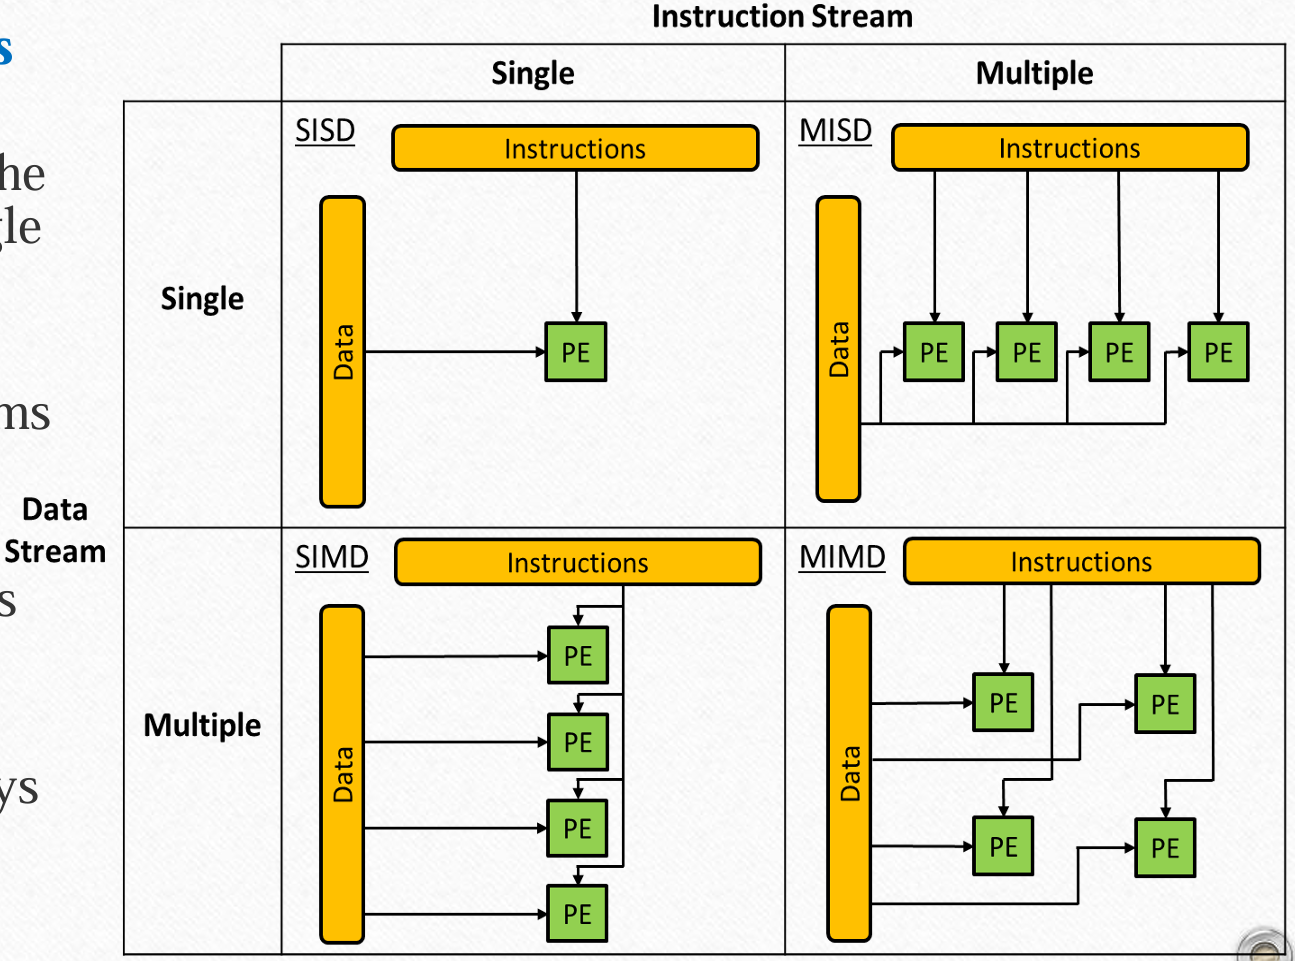
\includegraphics[width=0.95\columnwidth]{images/03/flynn.png}
      \caption{Flynn taxonomy}
      \label{fig:03/flynn}
   \end{figure}
\end{paracol}

\subsection{MIMD Architectures}
\begin{paracol}{2}
   \colfill
   A set of PEs (Processing Elements) simultaneously execute different instructions on different data streams. 
   Each processor can execute all instructions.
   This is the most common architecture for parallel systems.

   This architecture can be further classified considering memory organization and interconnection (between PE and MM) topologies.
   \colfill
   
   \switchcolumn

   \begin{figure}[htbp]
      \centering
      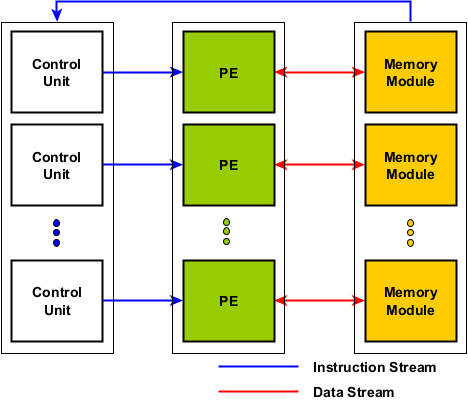
\includegraphics{images/03/mimd.png}
      \caption{MIMD architecture}
      \label{fig:03/mimd}
   \end{figure}
   
\end{paracol}

\newpage

\begin{paracol}{2}
   \begin{figure}[htbp]
      \centering
      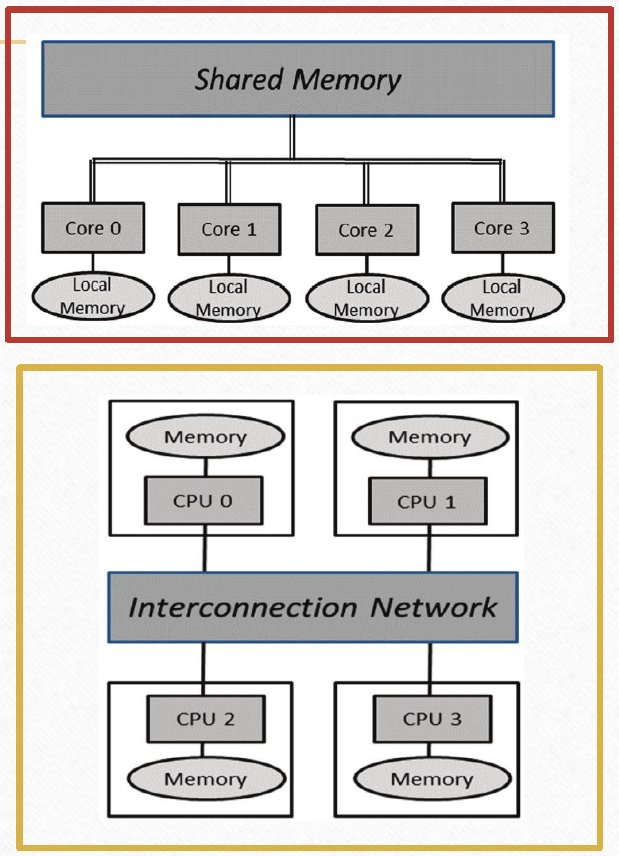
\includegraphics{images/03/mimd2.png}
      \caption{Classification based on memory}  
      \label{fig:03/mimd2}
   \end{figure}

   \switchcolumn

   \begin{itemize}
      \item \textbf{Shared Memory MIMD}: all processors share the same memory space, and can access it directly. This is the most common architecture for multi-core processors (\textit{``multiprocessors''}).
      \begin{itemize}
         \item \textbf{UMA (Uniform Memory Access)}: all processors access memory with the same latency.
         \note{SMP - Symmetric Multiprocessor}
         \item \textbf{NUMA (Non-Uniform Memory Access)}: processors access memory with different latencies.
         \note{\textit{Distributed Memory} architectures are inherently NUMA} 
      \end{itemize}
      \item \textbf{Distributed Memory MIMD}: each processor has its own memory space, and communicates with other processors through messages. This is the most common architecture for clusters.\\
      Interconnection may be based on Ethernet, InfiniBand, etc.
      \note{Historically called \textit{``multicomputers''}}
   \end{itemize}
\end{paracol}

\section{Classifying on cores count}
\begin{itemize}
   \item $\mathcal{O}(10^1 \div 10^2)$ cores, for a single multiprocessor chip (CMP)
   \item $\mathcal{O}(10^2 \div 10^3)$ cores, for a Shared Memory tightly-coupled multiprocessor
   \item $\mathcal{O}(10^3 \div 10^5)$ cores, for a Distributed Memory loosely-coupled multiprocessor (small to large compute clusters)
   \item $\mathcal{O}(10^5 \div 10^6)$ cores, top supercomputers (e.g. \textit{Leonardo @cineca})
\end{itemize}

\section{Programming Parallel Architectures}
\subsection{Shared-Memory}
In \textit{Shared-Memory} systems the emphasis is on the memory organization, meaning the memory hierarchy and processor-memory interconnections, aiming to reduce the \textit{``von Neumann bottleneck''}.
Critical aspects are \ul{cache coherence, memory consistency and thread synchronization}.

Programming models are based on \textit{thread-level parallelism} to exploit the phyisical shared memory by means of \textbf{Shared Variables} programming models (e.g. OpenMP, Pthreads, Cilk).

Caches shared among cores are used to reduce the latency of memory accesses, and to exploit the \textit{spatial locality} of data accesses, however they introduce the problem of \textit{cache coherence}, with respective issue (more on this later).

\subsection{Distributed-Memory}
In \textit{Distributed-Memory} systems the emphasis is on the interconnection network, aiming to reduce the \textit{``communication bottleneck''}, so reducing latency and increasing bandwidth.
Critical aspects are \ul{messaging protocols/libraries, routing}.

Here the only parallelism exploitable is \textit{process-level parallelism}, so the programming models are based on \textbf{message-passing} (e.g. MPI, POSIX socket, PVM).
\nl

Nowdays, each node is a CMP.
Depending on the network and some other aspects, we may further classify these systems in Clusters, Cloud, geographical distributed systems, etc.

We are interested in systems with \ul{high performance network topologies and homogeneous nodes}, like compute clusters.

A common example of application is the \textbf{Stencil Computation}, which is a common pattern in scientific computing, where each element of a matrix is computed as a function of its neighbors.

\subsection{Summary}
Distributed Memory systems are more scalable, costly and less energy efficient.

From the programming perspective, Shared Memory systems are easier to program and the physical shared memory can be used for fast communication between threads.
However, locking and synchronization are critical points deserving attention.

For what concerns Distributed Memory systems, the most important aspect is to reduce as much as possible the cost of communication (i.e. I/O), for instance overlapping computation and communication, reducing memory copies for I/O, using fast messaging protocols (e.g. RDMA).

\section{Suggested Readings}
\begin{itemize}
   \item 
   Chapter 1 - Section 1.2 - ``Parallelism Basics'' of Parallel Programming Concept and Practice book
   
   \item
   Chapter 3 - Section 3.2 - ``Flynn's Taxonomy'' of Parallel Programming Concept and Practice book
\end{itemize}